%!TEX root = ../clcxsj.tex

\chapter{附合导线近似平差程序设计}

虽然GPS的广泛应用使传统的控制测量趋于淘汰,但附合导线在一些工程中应用仍然非常广泛,如地铁、
隧道或建筑物密集的城区中的控制测量。在这些数据处理中,近似平差法由于不会受边角权的影响,能
最大程度的保持数据的真实性,仍然是数据检查的重要手段和数据处理的重要方法。

\section{程序功能简单分析}

\section{程序初步功能}

我们设计界面如图\ref{fig:ctUI01}所示:

\begin{figure}[htbp]
	\centering
	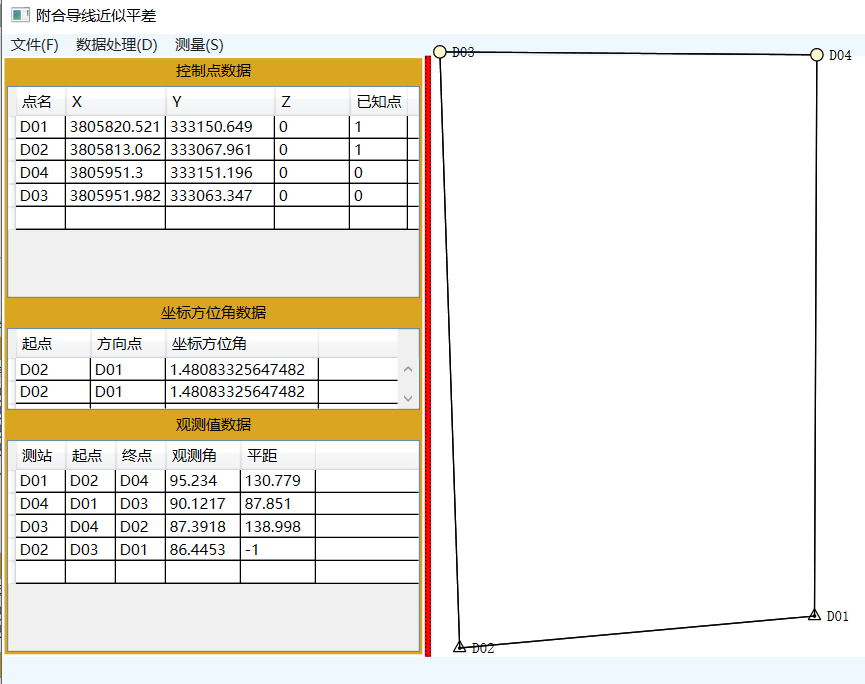
\includegraphics[scale=0.8]{connectingtraverse/ctUI01.png}
	\caption{附合导线界面功能图}
	\label{fig:ctUI01}
\end{figure}

\section{实现代码}

 \begin{lstlisting}[language=xml]
<Window x:Class="SurApp.MainWindow"
xmlns="http://schemas.microsoft.com/winfx/2006/xaml/presentation"
xmlns:x="http://schemas.microsoft.com/winfx/2006/xaml"
xmlns:local="clr-namespace:SurApp.models"
Title="附合导线近似平差" Height="350" Width="525"
WindowState="Maximized">

<DockPanel LastChildFill="True">
<Menu  x:Name="mainmenu" DockPanel.Dock="Top" Background="AliceBlue">
<MenuItem Header="文件(F)">
<MenuItem Header="新建附合导线..." Click="NewMenuItem_Click" />
<MenuItem Header="打开附合导线文件..." Click="OpenMenuItem_Click" />
<MenuItem Header="保存附合导线文件..."  Click="SaveMenuItem_Click" />
<Separator />
<MenuItem Header="导入文本数据" Click="ImportSPointMenuItem_Click"/>
<MenuItem Header="导出文本数据" Click="OutputSPointMenuItem_Click"/>
<Separator />
<MenuItem Header="导出为DXF文件" />
</MenuItem>

<MenuItem Header="数据处理(D)">
<MenuItem Header="附合导线平差" Click="AdjustMenuItem_Click" />
<MenuItem Header="平差成果" Click="AdjustResultMenuItem_Click" />
</MenuItem>

<MenuItem Header="测量(S)">
<MenuItem Header="角度弧度转换" Click="DMS2RADMenuItem_Click" />
<MenuItem Header="坐标方位角计算" Click="AzimuthMenuItem_Click" />
</MenuItem>
</Menu>
<StatusBar x:Name="statusBar" DockPanel.Dock="Bottom" Height="25"  Background="AliceBlue"/>
<Grid>
<Grid.ColumnDefinitions>
<ColumnDefinition Width="75*"/>
<ColumnDefinition Width="5"/>
<ColumnDefinition Width="170*"/>
</Grid.ColumnDefinitions>
<Border BorderThickness="2" Background="Goldenrod" Grid.Column="0">
<Grid x:Name="leftGrid" >
<Grid.RowDefinitions>
<RowDefinition Height="20"/>
<RowDefinition Height="100*"/>
<RowDefinition Height="20"/>
<RowDefinition Height="40*"/>
<RowDefinition Height="20"/>
<RowDefinition Height="100*"/>
</Grid.RowDefinitions>
<TextBlock Text="控制点数据" Grid.Row="0" TextAlignment="Center" Margin="2" />
<DataGrid x:Name="ctrPointDataGrid" Grid.Row="1" AutoGenerateColumns="False" Margin="2" ItemsSource="{Binding CtrPoints}" >
<DataGrid.Columns>
<DataGridTextColumn Header="点名" Binding="{Binding Name}" MinWidth="40"/>
<DataGridTextColumn Header="X" Binding="{Binding X , StringFormat={}{0:##0.###}}" MinWidth="60"/>
<DataGridTextColumn Header="Y" Binding="{Binding Y, StringFormat={}{0:##0.###}}" MinWidth="60" />
<DataGridTextColumn Header="Z" Binding="{Binding Z, StringFormat={}{0:##0.###}}" MinWidth="60"/>
<DataGridTextColumn Header="已知点" Binding="{Binding IsKnown}" MinWidth="30"/>
</DataGrid.Columns>
</DataGrid>

<TextBlock Text="坐标方位角数据" Grid.Row="2" TextAlignment="Center" Margin="2" />
<DataGrid x:Name="azimuthDataGrid" Grid.Row="3" AutoGenerateColumns="False" Margin="2" ItemsSource="{Binding KnownAzimuthes}" >
<DataGrid.Columns>
<DataGridTextColumn Header="起点" Binding="{Binding StartPnt.Name}" MinWidth="60"/>
<DataGridTextColumn Header="方向点" Binding="{Binding EndPnt.Name}" MinWidth="60"/>
<DataGridTextColumn Header="坐标方位角" Binding="{Binding Azimuth}" MinWidth="100" />
</DataGrid.Columns>
</DataGrid>

<TextBlock Text="观测值数据" Grid.Row="4" TextAlignment="Center" Margin="2"/>
<DataGrid x:Name="obsValueDataGrid" Grid.Row="5" AutoGenerateColumns="False"  Margin="2" ItemsSource="{Binding ObsValues}">
<DataGrid.Columns>
<DataGridTextColumn Header="测站" Binding="{Binding StnPnt.Name}" MinWidth="40"/>
<DataGridTextColumn Header="起点" Binding="{Binding StartPnt.Name}" MinWidth="40"/>
<DataGridTextColumn Header="终点" Binding="{Binding EndPnt.Name}" MinWidth="40" />
<DataGridTextColumn Header="观测角" Binding="{Binding DmsAngle}" MinWidth="60"/>
<DataGridTextColumn Header="平距" Binding="{Binding Distance}" MinWidth="60"/>
</DataGrid.Columns>
</DataGrid>

</Grid>
</Border>

<GridSplitter Background="Red" Width="5" Grid.Column="1" HorizontalAlignment="Stretch"/>

<Border BorderThickness="2" Grid.Column="2">
<local:DrawingCanvas x:Name="figureCanvas" SizeChanged="figureCanvas_SizeChanged">
<!--<Canvas.RenderTransform>
<TransformGroup>
<ScaleTransform x:Name="scaleTransform" ScaleX="1" ScaleY="-1" />
<TranslateTransform X ="0"  Y="{Binding ActualHeight, RelativeSource={RelativeSource AncestorType=Canvas}}" />
</TransformGroup>
</Canvas.RenderTransform>-->

<!--<Rectangle Height="50" Width="50" Fill="Red" Stroke="Blue" StrokeThickness="2" Canvas.Left="50" Canvas.Top="50" />

<Rectangle Height="50" Width="50" Fill="#CCCCCCFF" Stroke="Blue" StrokeThickness="2" Canvas.Left="50" Canvas.Top="50" >
<Rectangle.RenderTransform>
<TranslateTransform X="50" Y="50" />
</Rectangle.RenderTransform>
</Rectangle>-->
</local:DrawingCanvas>
</Border>
</Grid>
</DockPanel>

</Window>
 \end{lstlisting}

 \begin{lstlisting}[language=C]
using System;

namespace SurApp.models
{
[Serializable]
public class CtrPoint : ZXY.SPoint
{
private int isKnown = 0;

/// <summary>
/// 是否已知点(0:待定点, 1:已知点)
/// </summary>
public int IsKnown
	{
		get { return isKnown; }
		set
			{
				isKnown = value;
				this.RaisePropertyChange("IsKnown");
			}
	}

public CtrPoint() { }

public CtrPoint(string name, double x, double y, double z, int isKnown) : base(name, x, y, z)
{
		this.isKnown = isKnown;
	}

public override string ToString()
{
return string.Format("{0},{1},{2},{3}", Name, X, Y, Z);
}
}
}

using System;

namespace SurApp.models
{
[Serializable]
public class ObsValue : ZXY.NotificationObject
{
private CtrPoint stnPnt;
public CtrPoint StnPnt
	{
		get { return stnPnt; }
		set
			{
				stnPnt = value;
				this.RaisePropertyChange("StnPnt");
			}
	}

private CtrPoint startPnt;
public CtrPoint StartPnt
	{
		get { return startPnt; }
		set
			{
				startPnt = value;
				this.RaisePropertyChange("StartPnt");
			}
	}

private CtrPoint endPnt;
public CtrPoint EndPnt
	{
		get { return endPnt; }
		set
			{
				endPnt = value;
				this.RaisePropertyChange("EndPnt");
			}
	}

/// <summary>
///  观测角度值(单位:弧度)
/// </summary>
private double angleValue;

/// <summary>
/// 观测角度值(单位:弧度)
/// </summary>
public double AngleValue
	{
		get { return angleValue; }
		set
			{
				angleValue = value;
				this.RaisePropertyChange("DmsAngle");
				this.RaisePropertyChange("AngleValue");
			}
	}

/// <summary>
/// 观测角度值(单位:度分秒)
/// </summary>
public double DmsAngle
	{
		get { return ZXY.SMath.RAD2DMS(angleValue); }
		set
			{
				angleValue = ZXY.SMath.DMS2RAD(value);
				this.RaisePropertyChange("DmsAngle");
				this.RaisePropertyChange("AngleValue");
			}
	}


private double distance;
public double Distance
	{
		get { return distance; }
		set
			{
				distance = value;
				this.RaisePropertyChange("Distance");
			}
	}

public ObsValue() { }

public ObsValue(CtrPoint stnPnt, CtrPoint startPnt, CtrPoint endPnt,
double angleValue, double distance)
{
		this.stnPnt = stnPnt;
		this.startPnt = startPnt;
		this.endPnt = endPnt;
		this.DmsAngle = angleValue;
		this.distance = distance;
	}

private double vB; //角度改正数
public double VB
	{
		get { return vB; }
		set
			{
				vB = value;
				this.RaisePropertyChange("VB");
			}
	}

private double angleV; //改正后角度
public double AngleV
	{
		get { return angleV; }
		set
			{
				angleV = value;
				this.RaisePropertyChange("AngleV");
			}
	}

private double azimuth;
public double Azimuth
	{
		get { return azimuth; }
		set
			{
				azimuth = value;
				this.RaisePropertyChange("Azimuth");
			}
	}

private double dx;
public double DX
	{
		get { return dx; }
		set
			{
				dx = value;
				this.RaisePropertyChange("DX");
			}
	}

private double dy;
public double DY
	{
		get { return dy; }
		set
			{
				dy = value;
				this.RaisePropertyChange("DY");
			}
	}

private double vdx;
public double VDX
	{
		get { return vdx; }
		set
			{
				vdx = value;
				this.RaisePropertyChange("VDX");
			}
	}

private double vdy;
public double VDY
	{
		get { return vdy; }
		set
			{
				vdy = value;
				this.RaisePropertyChange("VDY");
			}
	}

public override string ToString()
{
return string.Format("{0},{1},{2},{3},{4}",
startPnt.Name, startPnt.Name, endPnt.Name,
DmsAngle, distance);
}
}
}

using System;
using System.Collections.Generic;
using System.Collections.ObjectModel;
using System.Windows.Media;
using ZXY;

namespace SurApp.models
{
/// <summary>
/// 用于已知边的坐标方位角信息
/// </summary>
[Serializable]
public class KnownAzimuth : NotificationObject
{
/// <summary>
/// 坐标方位角,单位:弧度
/// </summary>
public double azimuth;
public double Azimuth
	{
		get { return azimuth; }
		set
			{
				azimuth = value;
				this.RaisePropertyChange("Azimuth");
			}
	}

public CtrPoint startPnt; //坐标方位角的起点
public CtrPoint StartPnt
	{
		get { return startPnt; }
		set
			{
				startPnt = value;
				this.RaisePropertyChange("StartPnt");
			}
	}

public CtrPoint endPnt; //坐标方位角的方向点
public CtrPoint EndPnt
	{
		get { return endPnt; }
		set
			{
				endPnt = value;
				this.RaisePropertyChange("EndPnt");
			}
	}

public KnownAzimuth()
{
		startPnt = null;
		endPnt = null;
		azimuth = 0;
	}

public KnownAzimuth(CtrPoint startPnt, CtrPoint endPnt, double az)
{
		this.startPnt = startPnt;
		this.endPnt = endPnt;
		this.azimuth = az;
	}

public override string ToString()
{
if (startPnt == null || endPnt == null) return "~~~";
else
return string.Format("{0},{1},{2}", startPnt.Name, endPnt.Name, ZXY.SMath.RAD2DMS(azimuth));
}
}

[Serializable]
public class CtrNet : NotificationObject
{
private ObservableCollection<KnownAzimuth> knownAzimuthes = new ObservableCollection<KnownAzimuth>();
public ObservableCollection<KnownAzimuth> KnownAzimuthes
	{
		get { return knownAzimuthes; }
	}

private double m0 = 10; //中误差
private double fB;
private double FB; //角度闭合差的限差值
private double fx;
private double fy;
private double fs;

private double sumD;
private double K; // 1/K

//以下定义为绘图使用
private double minX;  //高斯坐标X的最小值xn
private double minY;  //高斯坐标Y的最小值yn
private double maxX; //高斯坐标X的最大值xm
private double maxY; //高斯坐标Y的最大值ym

private double maxVX; //屏幕坐标X的最大值
private double maxVY; //屏幕坐标Y的最大值

private double k;  //变换比例

private ObservableCollection<CtrPoint> ctrPoints =
new ObservableCollection<CtrPoint>();
public ObservableCollection<CtrPoint> CtrPoints
	{
		get { return ctrPoints; }
	}

private ObservableCollection<ObsValue> obsValues =
new ObservableCollection<ObsValue>();
public ObservableCollection<ObsValue> ObsValues
	{
		get { return obsValues; }
	}

/// <summary>
/// 正确的计算路线
/// </summary>
private List<ObsValue> route = new List<ObsValue>();

private bool isDirty = false;

public void ReadDataTextFile(string fileName)
{
using (System.IO.StreamReader sr = new System.IO.StreamReader(fileName))
{
string buffer;

//读入控制点数据
this.ctrPoints.Clear();
while (true)
{
		buffer = sr.ReadLine();
		if (string.IsNullOrEmpty(buffer)) break; //文件末尾或空行退出

		if (buffer[0] == '#') continue;

		string[] its = buffer.Split(new char[1] { ',' });
		if (its.Length != 4) continue; //不为四项控制点数据的继续,直到空行退出

		ctrPoints.Add(new CtrPoint(
		its[0].Trim(), // Name
		double.Parse(its[1]), //X
		double.Parse(its[2]), //Y
		double.Parse(its[3]), //H
		1)); //IsKnown
	}

//读入已知方位角信息:该节有可能不存在,也有可能有一条边,最多两条边
knownAzimuthes.Clear();
while (true)
{
		buffer = sr.ReadLine(); //由于是空行到此,所以继续往下读
		if (buffer == null) break; //文件末尾退出

		if (buffer == "" || buffer[0] == '#') continue; // 略过空行和注释行

		string[] its = buffer.Split(new char[1] { ',' });
		if (its.Length != 3) break; //数据项不为3,可能是角度观测值,退出当前

		KnownAzimuth ka = new KnownAzimuth();

		string ptName = its[0].Trim();
		ka.startPnt = GetCtrPoint(ptName);
		if (ka.startPnt == null)
		{
				ka.startPnt = new CtrPoint(ptName, 0, 0, 0, 0);//非已知点
				this.ctrPoints.Add(ka.startPnt);
			}

		ptName = its[1].Trim();
		ka.endPnt = GetCtrPoint(ptName);
		if (ka.endPnt == null)
		{
				ka.endPnt = new CtrPoint(ptName, 0, 0, 0, 0);//非已知点
				this.ctrPoints.Add(ka.endPnt);
			}

		ka.azimuth = ZXY.SMath.DMS2RAD(double.Parse(its[2]));
		knownAzimuthes.Add(ka);
	}

//读入观测值数据
this.obsValues.Clear();
while (true)
{
//此处可能由上不是3项数据的数据行退出,也有可能是文件末尾到此
//所以得先处理数据,后再读文本数据,否则,容易丢失数据
if (buffer == null) break; //文件末尾到此,继续退出
if (buffer == "" || buffer[0] == '#')//空行或正常的注释略过
{
buffer = sr.ReadLine();
continue;
}

string[] its = buffer.Split(new char[1] { ',' }); //进入正常的数据处理流程
if (its.Length == 5)
{
		string ptName = its[0].Trim();
		CtrPoint stnPnt = GetCtrPoint(ptName);
		if (stnPnt == null)
		{
				stnPnt = new CtrPoint(ptName, 0, 0, 0, 0);//非已知点
				this.ctrPoints.Add(stnPnt);
			}

		ptName = its[1].Trim();
		CtrPoint startPnt = GetCtrPoint(ptName);
		if (startPnt == null)
		{
				startPnt = new CtrPoint(ptName, 0, 0, 0, 0);//非已知点
				this.ctrPoints.Add(startPnt);
			}

		ptName = its[2].Trim();
		CtrPoint endPnt = GetCtrPoint(ptName);
		if (endPnt == null)
		{
				endPnt = new CtrPoint(ptName, 0, 0, 0, 0);//非已知点
				this.ctrPoints.Add(endPnt);
			}

		obsValues.Add(new ObsValue(
		stnPnt, startPnt, endPnt,
		double.Parse(its[3]), //AngleValue
		double.Parse(its[4]))); //Distance
	}

buffer = sr.ReadLine();
}
}
}

public void WriteDataTextFile(string fileName)
{
		using (System.IO.StreamWriter sw = new System.IO.StreamWriter(fileName))
		{
				sw.WriteLine("# Name, X, Y, Z");
				foreach (var pt in this.ctrPoints)
				{
						if(pt.IsKnown == 1) sw.WriteLine( pt );
					}

				sw.WriteLine();
				sw.WriteLine("# StartPnt, EndPnt, Azimuth");
				foreach (var az in this.knownAzimuthes)
				{
						sw.WriteLine( az );
					}

				sw.WriteLine();
				sw.WriteLine("# Station, StartPnt, EndPnt, Angle, Distance");
				foreach (var obs in this.ObsValues)
				{
						sw.WriteLine( obs );
					}
			}
	}


private ObsValue SearchStartObsValue()
{
		/**
		* 搜索起始边,首先:搜索直接给定的坐标方位角
		* 其次:上述搜索不成立的情况,搜索:测站点与后视点均为已知点的观测值
		* 再次:反向搜索:测站点与后视点均为已知点的观测值
		* */
		ObsValue obs = null;

		if (this.knownAzimuthes.Count > 0)
		{
				foreach (var azi in this.knownAzimuthes)
				{
						if (azi.endPnt.IsKnown == 1)
						{
								foreach (var it in obsValues)
								{
										if (it.StartPnt == azi.startPnt && it.StnPnt == azi.endPnt)
										{
												obs = it;
												return obs;
											}
									}
							}
					}
			}
		else if (this.knownAzimuthes.Count == 0)
		{
				foreach (var it in obsValues)
				{
						double az = 0;

						if (it.StartPnt.IsKnown == 1 && it.StnPnt.IsKnown == 1)
						{
								az = ZXY.SMath.Azimuth(it.StartPnt.X, it.StartPnt.Y, it.StnPnt.X, it.StnPnt.Y);
								this.knownAzimuthes.Add(new KnownAzimuth(it.StartPnt, it.StnPnt, az));
								obs = it;
							}

						if (it.StnPnt.IsKnown == 1 && it.EndPnt.IsKnown == 1)
						{
								az = ZXY.SMath.Azimuth(it.StnPnt.X, it.StnPnt.Y, it.EndPnt.X, it.EndPnt.Y);
								this.knownAzimuthes.Add(new KnownAzimuth(it.StnPnt, it.EndPnt, az));
							}
					}
			}
		return obs;
	}


/// <summary>
/// 递归搜索观测值obs0的下一条边
/// </summary>
/// <param name="obs0">当前观测值</param>
/// <returns>1:附合导线, -1:不构成附合导线</returns>
private int SearchObsValue(ObsValue obs0)
{
//传进来的第一条边应为起始边
ObsValue obsi = null;

foreach (var it in obsValues)
{
if (it == obs0) continue;

if (obs0.StnPnt == it.StartPnt && obs0.EndPnt == it.StnPnt)  //满足条件的下一条边
{
obsi = it;
break;
}
}

if (obsi == null) return -1;//没找到这样的边

this.route.Add(obsi);
if (obsi.StnPnt.IsKnown == 1 && obsi.EndPnt.IsKnown == 1) //附合到另一条已知边了,退出
{
return 1;
}
else
SearchObsValue(obsi); //递归继续寻找下一条这样的边

return 0;
}


/// <summary>
/// 搜索正确的计算路线
/// </summary>
/// <returns>是否成功</returns>
public bool SearchCalRoute()
{
		ObsValue obs0 = SearchStartObsValue();
		if (obs0 == null) return false;

		route.Clear(); //清空搜索线路

		route.Add(obs0);
		SearchObsValue(obs0);
		return true;
	}

/// <summary>
/// 简易平差
/// </summary>
/// <returns>0:成功</returns>
public int Adjust()
{
		/*
		1. 求起始边: 后视->测站 的方位角
		求末边:测站->前视 的方位角
		2. 计算角度闭合差fB,FB
		3. 改正角度值
		4. 推算各边坐标方位角
		5. 计算各边的坐标增量
		6.计算fx, fy, fs, 1/K
		7.计算改正后的坐标增量
		8.计算各点的坐标值
		*/
		if (this.obsValues.Count == 0) return -1; //观测值为空

		if (SearchCalRoute() == false) return -2; //搜索不到正确的附合路线

		double az0 = this.knownAzimuthes[0].azimuth;
		CtrPoint startPnt0 = this.knownAzimuthes[0].startPnt;
		CtrPoint stnPnt0 = this.knownAzimuthes[0].endPnt;

		double azn = this.knownAzimuthes[1].azimuth;
		CtrPoint stnPntn = this.knownAzimuthes[1].startPnt;
		CtrPoint endPntn = this.knownAzimuthes[1].endPnt;

		double azi = az0;
		double n = route.Count;
		foreach (var obs in route) //foreach (var obs in this.ObsValues)
		{
				obs.Azimuth = azi + obs.AngleValue + Math.PI;
				if (obs.Azimuth >= 2 * Math.PI) obs.Azimuth -= 2 * Math.PI;
				if (obs.Azimuth < 0) obs.Azimuth += 2 * Math.PI;

				azi = obs.Azimuth;
			}

		fB = azi - azn; //单位:弧度
		FB = m0 * 2 * Math.Sqrt(n); //单位:秒

		//改正角度,推算各边改正后的方位角
		azi = az0;
		double vi = -fB / n;
		foreach (var obs in route) //foreach (var obs in this.ObsValues)
		{
				obs.VB = vi;
				obs.AngleV = obs.AngleValue + obs.VB;
				obs.Azimuth = azi + obs.AngleV + Math.PI;
				if (obs.Azimuth >= 2 * Math.PI) obs.Azimuth -= 2 * Math.PI;
				if (obs.Azimuth < 0) obs.Azimuth += 2 * Math.PI;
				azi = obs.Azimuth;
			}

		//计算各边的坐标增量
		double sumDX = 0, sumDY = 0;
		sumD = 0;
		foreach (var obs in route) //foreach (var obs in this.ObsValues)
		{
				if (obs.Distance <= 0) continue;

				obs.DX = obs.Distance * Math.Cos(obs.Azimuth);
				obs.DY = obs.Distance * Math.Sin(obs.Azimuth);
				sumDX += obs.DX;
				sumDY += obs.DY;
				sumD += obs.Distance;
			}
		fx = stnPnt0.X + sumDX - stnPntn.X;
		fy = stnPnt0.Y + sumDY - stnPntn.Y;
		fs = Math.Sqrt(fx * fx + fy * fy);
		K = sumD / fs;

		//改正坐标增量,计算各点坐标
		foreach (var obs in route) //foreach (var obs in this.ObsValues)
		{
				if (obs.Distance <= 0) continue;

				obs.VDX = -fx / sumD * obs.Distance;
				obs.VDY = -fy / sumD * obs.Distance;

				obs.EndPnt.X = obs.StnPnt.X + obs.DX + obs.VDX;
				obs.EndPnt.Y = obs.StnPnt.Y + obs.DY + obs.VDY;
			}

		return 0;
	}

private CtrPoint GetCtrPoint(string pointName)
{
		foreach (var pt in this.ctrPoints)
		{
				if (pt.Name == pointName)
				return pt;
			}

		return null;
	}

public void OnDraw(DrawingCanvas canvas)
{
		if (this.ctrPoints.Count < 1) return;

		GetGaussXySize();

		maxVX = canvas.ActualWidth-20;
		maxVY = canvas.ActualHeight;

		double kx = maxVX / (maxY - minY);
		double ky = maxVY / (maxX - minX);
		k = kx <= ky ? kx : ky;

		canvas.ClearAll(); //先清除屏幕

		//画观测值
		double x0, y0, x1, y1, x2, y2; //画直线的两个端点
		foreach (var it in this.obsValues)
		{
				if (it.StnPnt.X <= 0 && it.StnPnt.Y <= 0) continue; //略过坐标为0的点
				GaussXyToViewXy(it.StnPnt.X, it.StnPnt.Y, out x0, out y0);

				if (it.StartPnt.X > 0 && it.StartPnt.Y > 0)
				{
						GaussXyToViewXy(it.StartPnt.X, it.StartPnt.Y, out x1, out y1);
						canvas.DrawLine(x1, y1, x0, y0, Brushes.Black, 1);
					}

				if (it.EndPnt.X > 0 && it.EndPnt.Y > 0)
				{
						GaussXyToViewXy(it.EndPnt.X, it.EndPnt.Y, out x2, out y2);
						canvas.DrawLine(x0, y0, x2, y2, Brushes.Black, 1);
					}
			}

		//再画控制点
		foreach (var pt in this.ctrPoints)
		{
				if (pt.X <= 0 && pt.Y <= 0) continue; //排除坐标为0的点

				GaussXyToViewXy(pt.X, pt.Y, out x0, out y0);
				if(pt.IsKnown == 1)
				canvas.DrawKnCtrPnt(x0, y0, Brushes.Black, 1);
				else
				canvas.DrawCtrPnt(x0, y0, Brushes.Black, 1);
				canvas.DrawText(pt.Name, x0 + 10, y0 - 7);
			}
	}

private void GaussXyToViewXy(double xt, double yt, out double xp, out double yp)
{
		//xp = x0 + kx(yt - yn);
		//yp = y1 - (y0 + ky * (xt - xn));
		// x0 = y0 =0 且 kx = ky =k, 故以上公式简化为:

		xp = 5 + k * (yt - minY); //x0 = 5;
		yp = maxVY - (5 + k * (xt - minX)); //y0=5;
	}

private void GetGaussXySize()
{
minX = this.ctrPoints[0].X; minY = this.ctrPoints[0].Y;
maxX = this.ctrPoints[0].X; maxY = this.ctrPoints[0].Y;

for (int i = 1; i < this.ctrPoints.Count; i++) //如果只有一个点,由循环条件知,不会执行循环体
{
if (this.ctrPoints[i].X <= 0 && this.ctrPoints[i].Y <= 0) continue;

if (this.ctrPoints[i].X < minX) minX = this.ctrPoints[i].X;
if (this.ctrPoints[i].Y < minY) minY = this.ctrPoints[i].Y;

if (this.ctrPoints[i].X > maxX) maxX = this.ctrPoints[i].X;
if (this.ctrPoints[i].Y > maxY) maxY = this.ctrPoints[i].Y;
}

//针对一个点或点范围较小的情况,进行范围扩展
if (minX + 10 > maxX) { maxX = minX + 10; minX = maxX - 20; }
if (minY + 10 > maxY) { maxY = minY + 10; minY = maxY - 20; }
}
}
}

using System.Globalization;
using System.Windows;
using System.Windows.Media;

namespace SurApp.models
	{
		public class DrawingCanvas : System.Windows.Controls.Canvas
			{
				private VisualCollection visuals;

				public DrawingCanvas()
				{
						visuals = new VisualCollection(this);
					}

				//获取Visual的个数
				protected override int VisualChildrenCount
					{
						get { return visuals.Count; }
					}

				//获取Visual
				protected override Visual GetVisualChild(int index)
				{
						return visuals[index];
					}

				//添加Visual
				public void AddVisual(Visual visualObject)
				{
						visuals.Add( visualObject );
					}

				//删除Visual
				public void RemoveVisual(Visual visualObject)
				{
						base.RemoveLogicalChild(visualObject);
					}

				//命中测试
				public DrawingVisual GetVisual(System.Windows.Point point)
				{
						HitTestResult hitResult = VisualTreeHelper.HitTest(this, point);
						return hitResult.VisualHit as DrawingVisual;
					}

				public void ClearAll()
				{
						this.visuals.Clear();
					}


				//使用DrawVisual画Polyline
				public void DrawLine(double x0, double y0, double x1, double y1,  Brush color, double thinkness)
				{
						DrawingVisual visualLine = new DrawingVisual();
						DrawingContext dc = visualLine.RenderOpen();
						Pen pen = new Pen(color, thinkness);
						pen.Freeze();  //冻结画笔,这样能加快绘图速度
						dc.DrawLine(pen, new Point(x0, y0),  new Point(x1, y1) );

						dc.Close();
						visuals.Add(visualLine);
					}

				public void DrawText(string text, double x, double y)
				{
						DrawingVisual visualText = new DrawingVisual();
						DrawingContext dc = visualText.RenderOpen();
						Typeface tp = new Typeface(new FontFamily("宋体"), FontStyles.Normal, FontWeights.Normal, FontStretches.Normal);
						FormattedText ft = new FormattedText(text, CultureInfo.CurrentCulture,
						FlowDirection.LeftToRight, tp, 12, Brushes.Black);
						dc.DrawText(ft, new Point(x, y) );
						dc.Close();
						visuals.Add( visualText );
					}

				//使用DrawVisual画Circle,用作控制点
				public void DrawCtrPnt(double x, double y,  Brush color, double thinkness)
				{
						DrawingVisual visualCircle = new DrawingVisual();
						DrawingContext dc = visualCircle.RenderOpen();
						Pen pen = new Pen(color, thinkness);
						pen.Freeze();  //冻结画笔,这样能加快绘图速度
						dc.DrawEllipse(Brushes.LemonChiffon,  pen,  new Point(x, y),  5, 5);
						dc.Close();
						visuals.Add(visualCircle);
					}

				//使用DrawVisual画Circle,用作控制点
				public void DrawKnCtrPnt(double x, double y, Brush color, double thinkness)
				{
						DrawingVisual visualCircle = new DrawingVisual();
						DrawingContext dc = visualCircle.RenderOpen();
						Pen pen = new Pen(color, thinkness);
						pen.Freeze();  //冻结画笔,这样能加快绘图速度
						dc.DrawEllipse(Brushes.Black, pen, new Point(x, y), 1, 1);
						dc.DrawLine(pen, new Point(x-5, y+2.9), new Point(x+5, y+2.9));
						dc.DrawLine(pen, new Point(x + 5, y + 2.9), new Point(x, y - 5.8));
						dc.DrawLine(pen, new Point(x, y - 5.8), new Point(x - 5, y + 2.9));
						dc.Close();
						visuals.Add(visualCircle);
					}
			}
	}

 \end{lstlisting}
